% Author: Ben Champion <bwc3252@rit.edu>
% Main LaTeX file for Lenfest Community Weekend 2019 Presentation

\documentclass{beamer}

\usetheme{Amsterdam}

\usepackage{caption}

\begin{document}
\title{Astrophysical Parameter Inference with Gravitational Wave and Electromagnetic Data Channels}
\author{Ben Champion}
\institute{Rochester Institute of Technology \\ Center for Computational Relativity and Gravitation}

% logos
\titlegraphic{
\includegraphics[width=6cm]{Images/RIT_RGB_hor_k}\hspace*{2cm}~%
   
\includegraphics[width=2cm]{Images/ccrg_logo}
}

\date{
  \today
}

\frame{
  \titlepage
}

\frame{ \frametitle{Table of contents}
  \tableofcontents
}

\section{Introduction}

\frame{ \frametitle{Classical Physics}
  \begin{itemize}
    \item Late 1600s - Newton's law of universal gravitation:
    \begin{figure}
      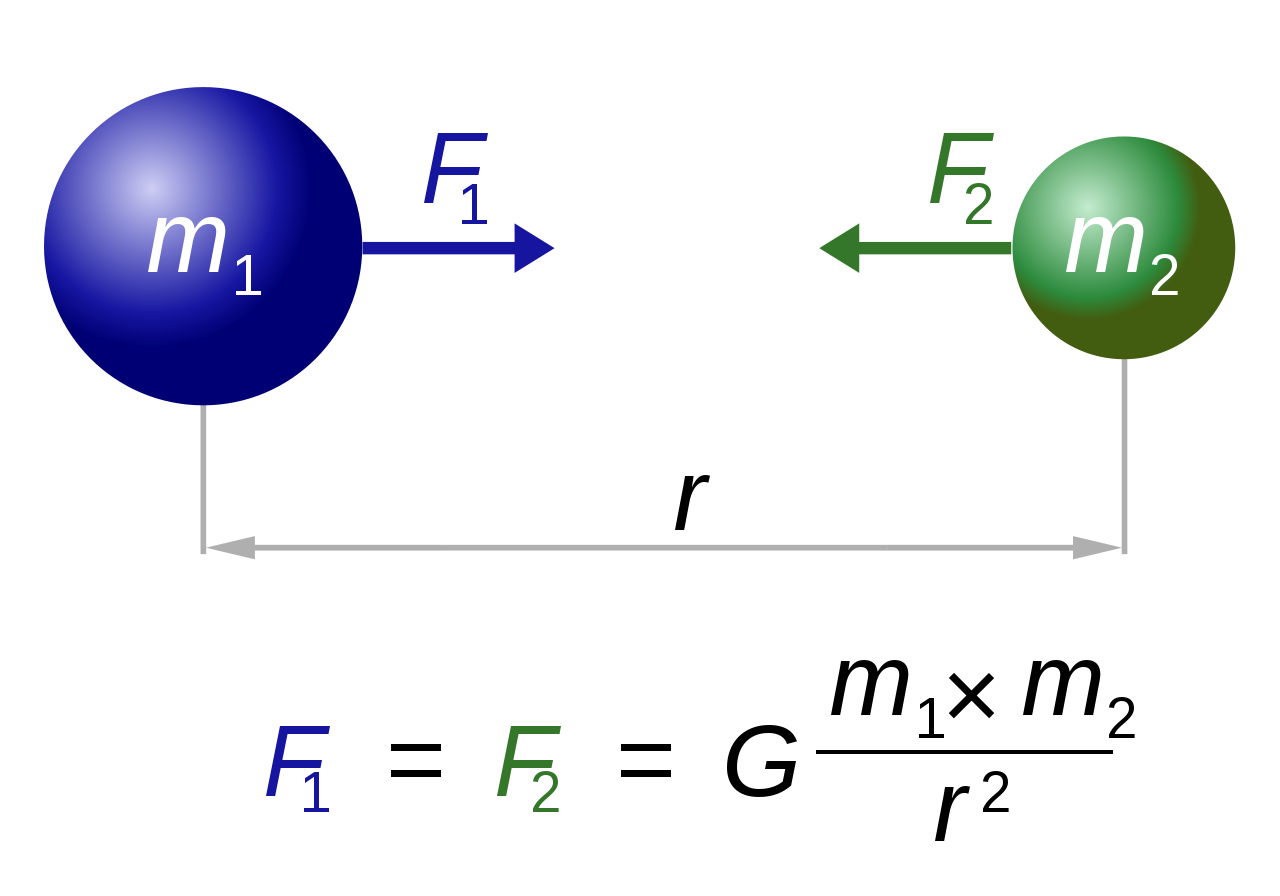
\includegraphics[width=1.75in]{Images/universal_gravitation}
      \caption*{\fontsize{8pt}{10pt}\selectfont Image by Dennis Nilsson}
    \end{figure}
  \end{itemize}
}

\frame{ \frametitle{Special Relativity}
  \begin{columns}[c]
    \column{3.0in}
    \begin{itemize}
      \item 1905 - Einstein's theory of Special Relativity \pause
      \begin{itemize}
        \item The speed of light is independent of the motion of the observer \pause
        \item Consequences include length contraction, time dilation, etc. \pause
        \item Shortcoming: only applies to inertial (non-accelerating) reference frames \pause
      \end{itemize}
    \end{itemize}
    \column{1.5in}
    \begin{figure}
      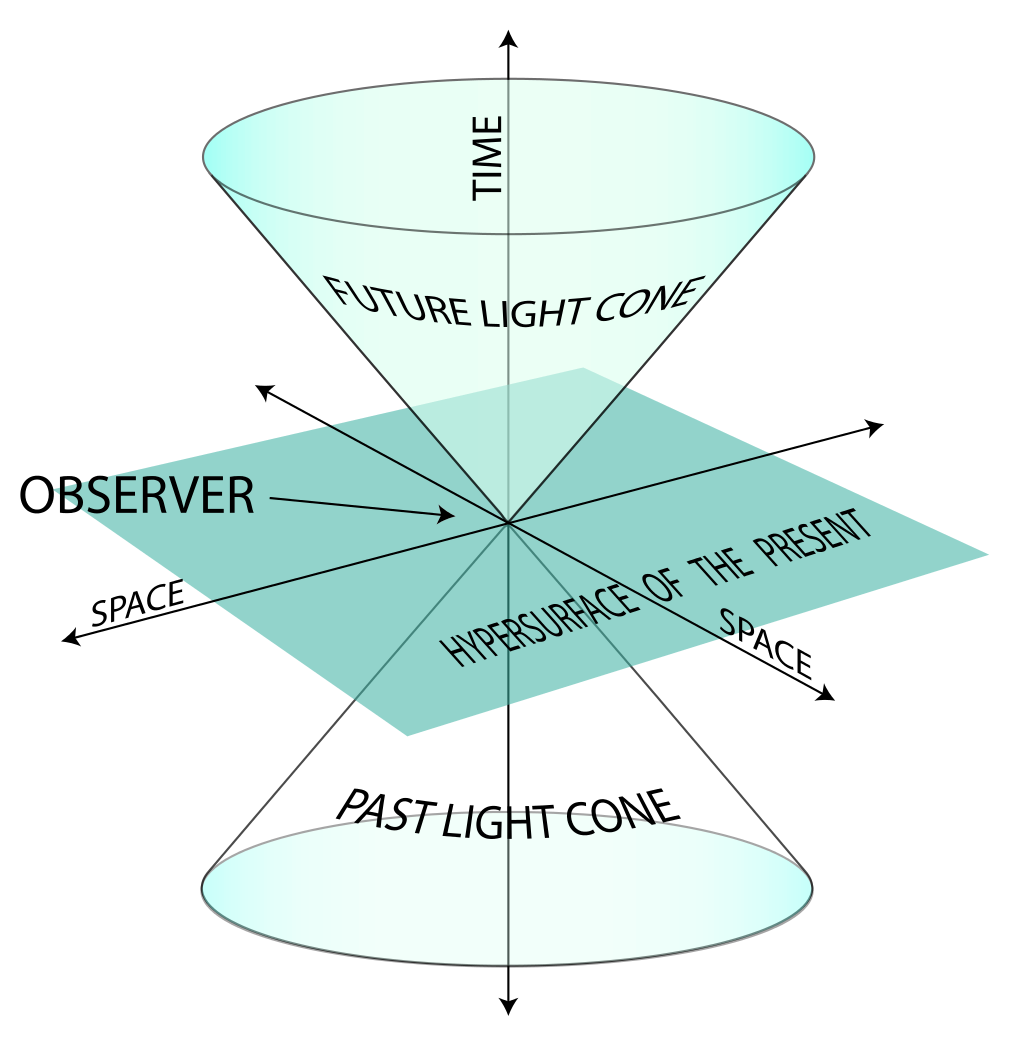
\includegraphics[width=\linewidth]{Images/world_line}
      \caption*{\fontsize{8pt}{10pt}\selectfont Lightcone: the path through spacetime that a single flash of light, traveling in all directions, would take (image by K. Aainsqatsi)}
    \end{figure}
  \end{columns}
}

\frame{ \frametitle{Special Relativity}
  Classically, for an event with coordinates $(t, x)$ as measured by a stationary observer and $(t', x')$ as measured by an observer moving with velocity $v$:

  \begin{align*}
    t' &= t  \\
    x' &= x - vt
  \end{align*}

  \pause

  However, according to Special Relativity:

  \begin{align*}
    t' &= \gamma (t - \frac {vx} {c^2}) \\
    x' &= \gamma (x - vt) \\
    \text{where } \gamma &= \frac {1} {\sqrt{1 - \frac {v^2} {c^2}}}
  \end{align*}

  }

\frame{ \frametitle{General Relativity}
  \begin{itemize}
    \item 1915 - Einstein's theory of General Relativity \pause
    \begin{itemize}
      \item Einstein's efforts to include acceleration and external forces (e.g. gravity) in relativity resulted in his theory of General Relativity \pause
      \item Objects with mass change the geometry of spacetime itself \pause
    \end{itemize}
    \item Einstein field equations: describe relationship between four-dimensional spacetime and and the energy-momentum contained in that spacetime \pause \\
    \begin{align*}
      R_{\mu v} - \frac {1} {2} R g_{\mu v} + \Lambda g_{\mu v} = \frac {8 \pi G} {c^4} T_{\mu v}
    \end{align*}
  \end{itemize}
}

\frame{ \frametitle{Einstein Field Equations}
  \begin{columns}[c]
    \column{2.5in}
    \begin{align*}
      R_{\mu \nu} - \frac {1} {2} R g_{\mu \nu} + \Lambda g_{\mu \nu} = \frac {8 \pi G} {c^4} T_{\mu \nu}
    \end{align*}
    \begin{tabular}{l l}
      $R_{\mu v}$   & Ricci curvature tensor \\
      $R$           & scalar curvature \\
      $g_{\mu \nu}$ & metric tensor \\
      $\Lambda$     & cosmological constant \\
      $T_{\mu \nu}$ & stress-energy tensor
    \end{tabular}
    \column{2.0in}
    \begin{figure}
      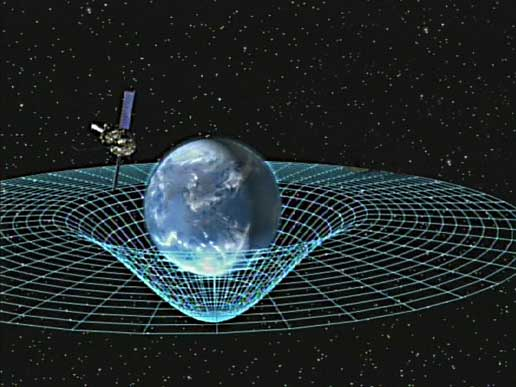
\includegraphics[width=\linewidth]{Images/general_relativity}
    \end{figure}
  \end{columns}
}

\frame{ \frametitle{Consequences of General Relativity}
  \begin{columns}[c]
    \column{2.5in}
    \begin{itemize}
      \item Black holes \pause
      \item Bending of light around massive objects \pause
      \item Gravitational time dilation \pause
      \item Gravitational waves \pause
    \end{itemize}
    \column{2.5in}
    \begin{figure}
      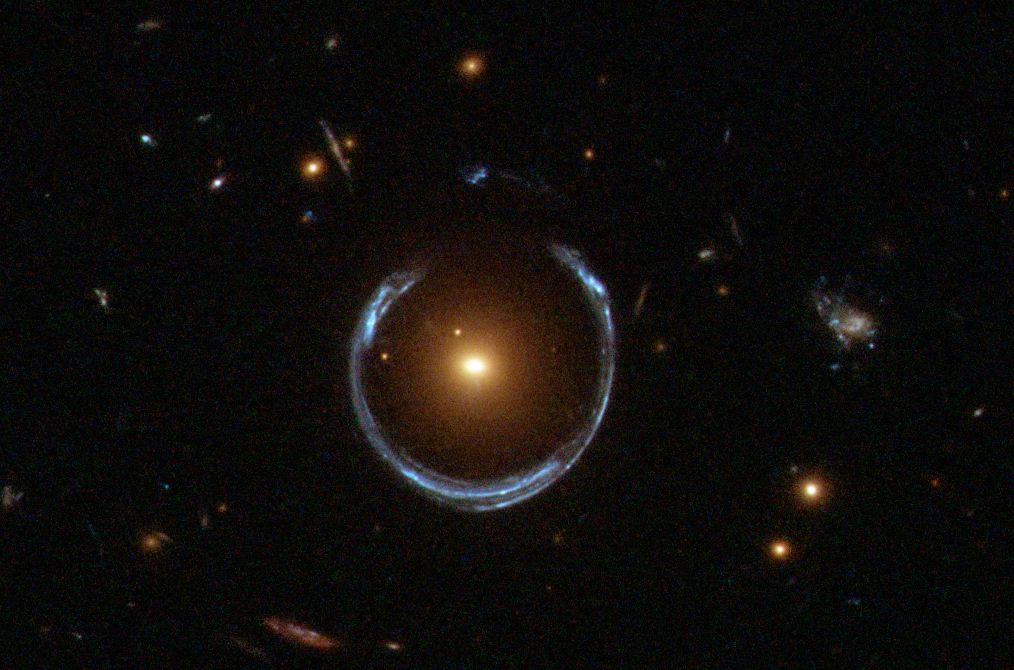
\includegraphics[width=\linewidth]{Images/lensing}
      \caption*{A galaxy bends the light from a more distant galaxy, resulting in \textit{gravitational lensing}}
    \end{figure}
  \end{columns}
}

\frame{ \frametitle{Gravitational Waves}
  \begin{itemize}
    \item Objects with mass cause distortions in spacetime \pause
    \item Motion involving a changing acceleration produces gravitational waves \pause
    \begin{itemize}
      \item (assuming this motion does not involve spherical or rotational symmetry) \pause
    \end{itemize}
    \item The gravitational waves produced by most objects are too small to detect \pause
    \item Gravitational waves produced by merging black holes or neutron stars are large enough to detect
  \end{itemize}
}

\frame{ \frametitle{Gravitational Wave Interferometry}
  \begin{columns}[c]
    \column{2.5in}
    \begin{itemize}
      \item LIGO - the Laser Interferometer Gravitational Wave Observatory - has two detectors
    \end{itemize}
    \begin{figure}
      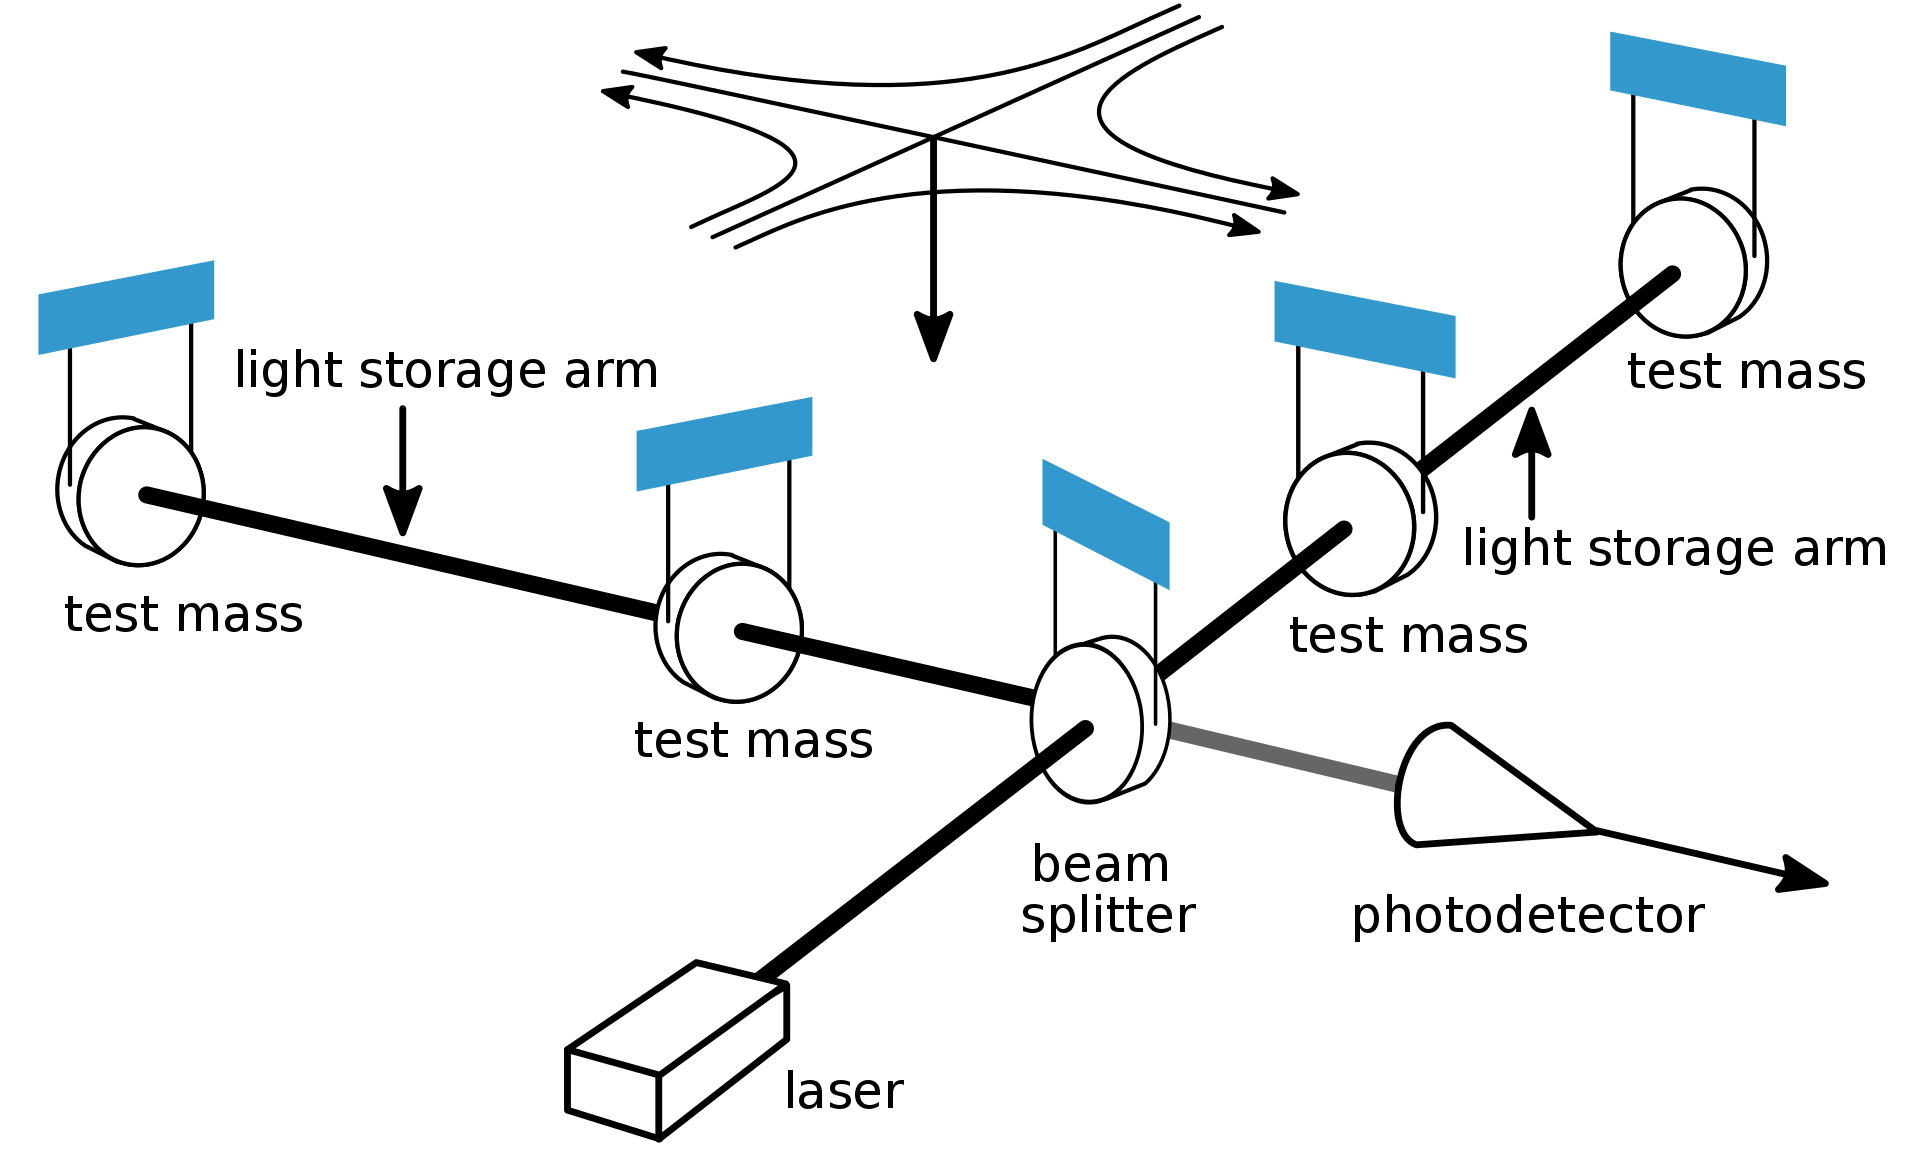
\includegraphics[width=2.0in]{Images/interferometer}
      \caption*{\fontsize{8pt}{10pt}\selectfont Image by Barry Barish}
    \end{figure}
    \pause
    \column{2.25in}
    \begin{itemize}
      \item As a gravitational wave passes, one arm stretches and the other shrinks \pause
      \item When the arms are the same length, the interference pattern detected is completely destructive \pause
      \item When one arm is longer than the other, it takes light more time to travel down that arm, resulting in a detectable interference pattern
    \end{itemize}
  \end{columns}
}

\frame{ \frametitle{Gravitational Wave Detections}
  \begin{figure}
    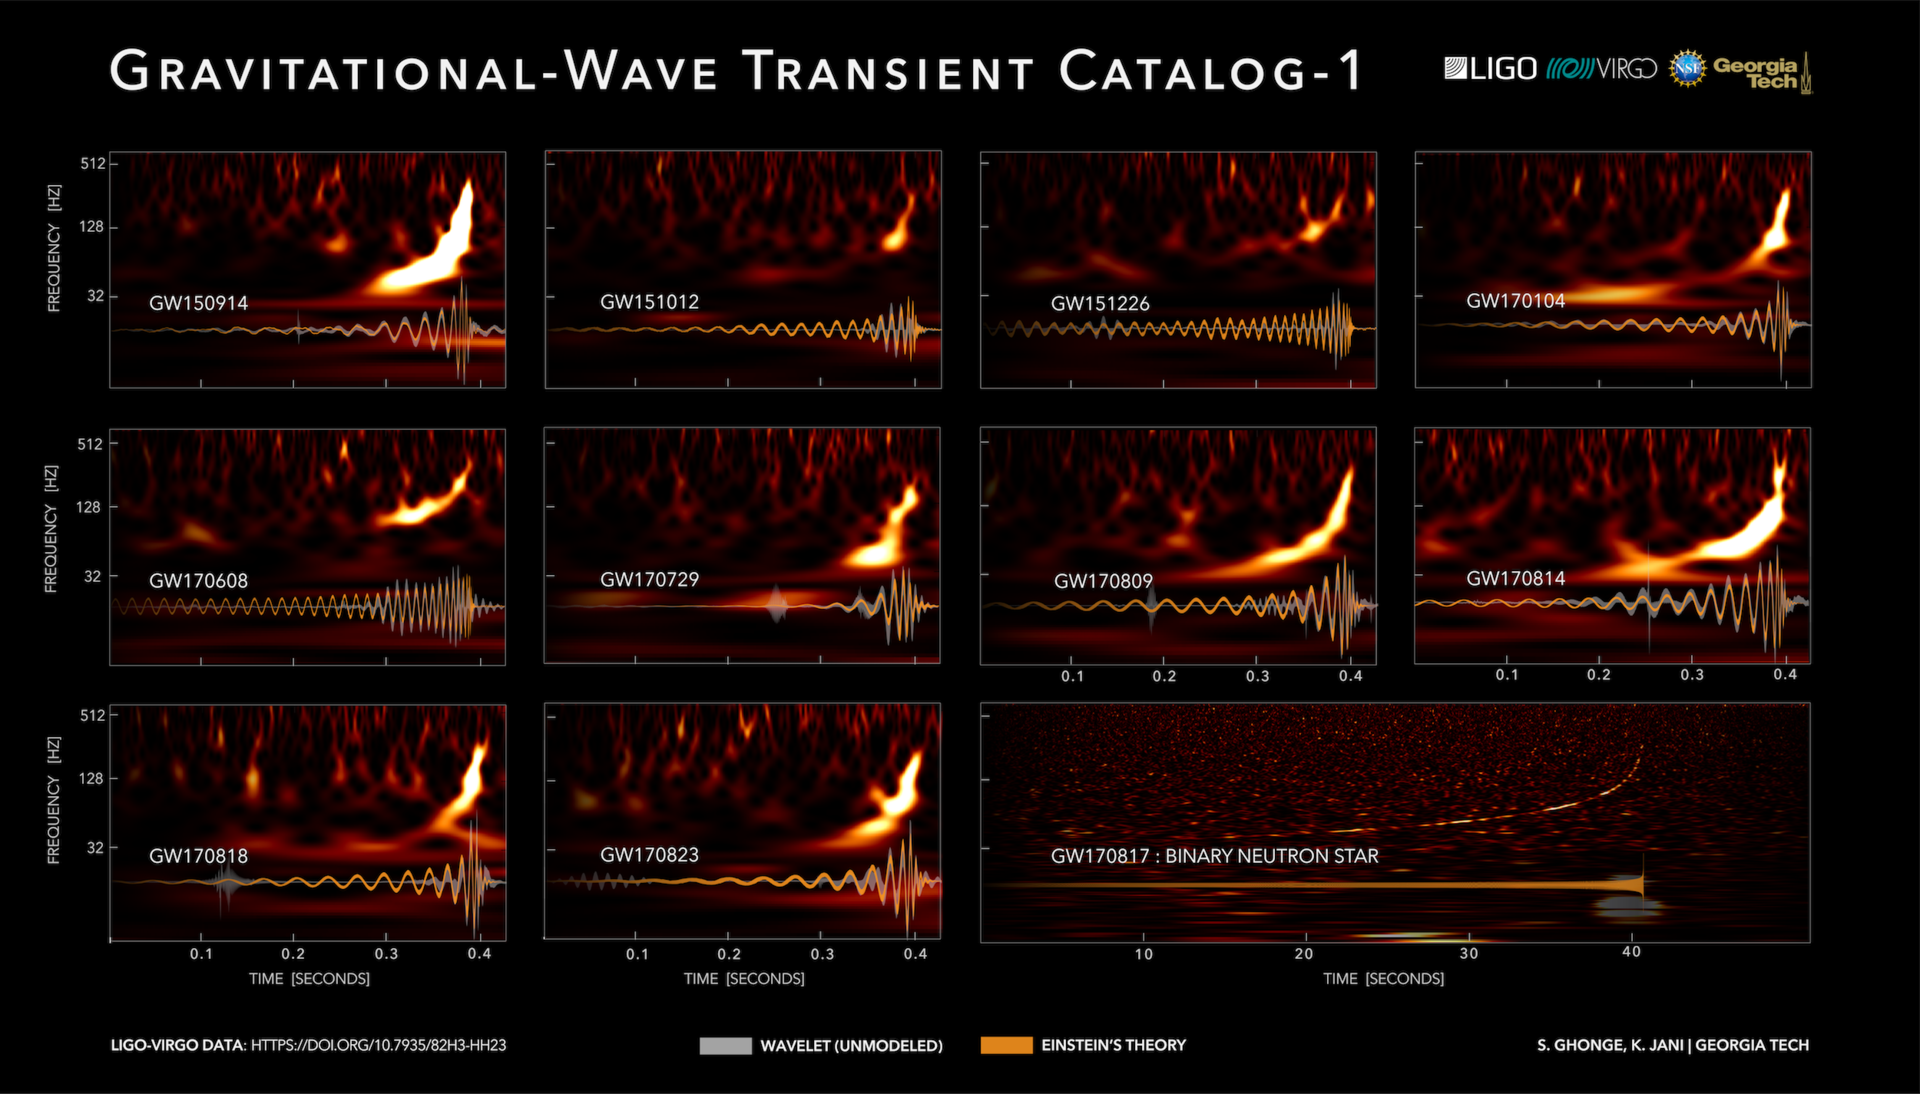
\includegraphics[width=\linewidth]{Images/detections}
    \caption*{\fontsize{8pt}{10pt}\selectfont Image by LIGO/Virgo/Georgia Tech/S. Ghonge \& K. Jani}
  \end{figure}
}

\section{Gravitational Wave PE}

\frame{ \frametitle{What is Parameter Estimation?}
  \begin{itemize}
    \item Estimation of astrophysical source parameters from observations \pause
    \begin{itemize}
      \item Intrinsic parameters: \pause
      \begin{itemize}
        \item Mass \pause
        \item Spin \pause
        \item Compactness (for neutron stars) \pause
      \end{itemize}
      \item Extrinsic parameters: \pause
      \begin{itemize}
        \item Sky location \pause
        \item Distance \pause
        \item Orientation \pause
      \end{itemize}
    \end{itemize}
  \item Goal is to recover a \textit{posterior distribution} of parameters, using theoretical models that give waveforms as functions of these parameters
  \end{itemize}
}

\frame{ \frametitle{Bayes' Theorem and Model Likelihoods}
  For a vector of unknown parameters $\vec \theta$, proposed waveform model $H$, and set of observations $\{d\}$, Bayes' Theorem gives the \textit{probability density function} of $\vec \theta$ as
  \begin{align*}
    p(\vec \theta | \{d\}, H) = \frac {p(\vec \theta | H) p(\{d\} | \vec \theta, H)} {p(\{d\} | H)}
  \end{align*} \pause
  \begin{itemize}
    \item $p(\vec \theta | H)$ is the \textit{prior} distribution of $\vec \theta$ \pause
    \item $p(\{d\} | \vec \theta, H)$ is the \textit{likelihood function} - the likelihood of observing $\{d\}$ given $\vec \theta$ and $H$ \pause
    \begin{itemize}
      \item Function of residuals - differences between model and data
    \end{itemize}
  \end{itemize}
}

\frame{ \frametitle{Adaptive Sampling}
  \begin{itemize}
    \item Sampling the parameter space - the possible values of $\vec \theta$ - and calculating the probability density at each point allows us to draw conclusions about the parameters \pause
    \item Problem: parameter spaces are high-dimensional and likelihood calculations are computationally expensive \pause
    \item Solution: Sample parameter space \textit{adaptively} - that is, focus on parts of the parameter space with high likelihoods
  \end{itemize}
}

\frame{ \frametitle{Posterior Distribution Example}
  \begin{figure}
    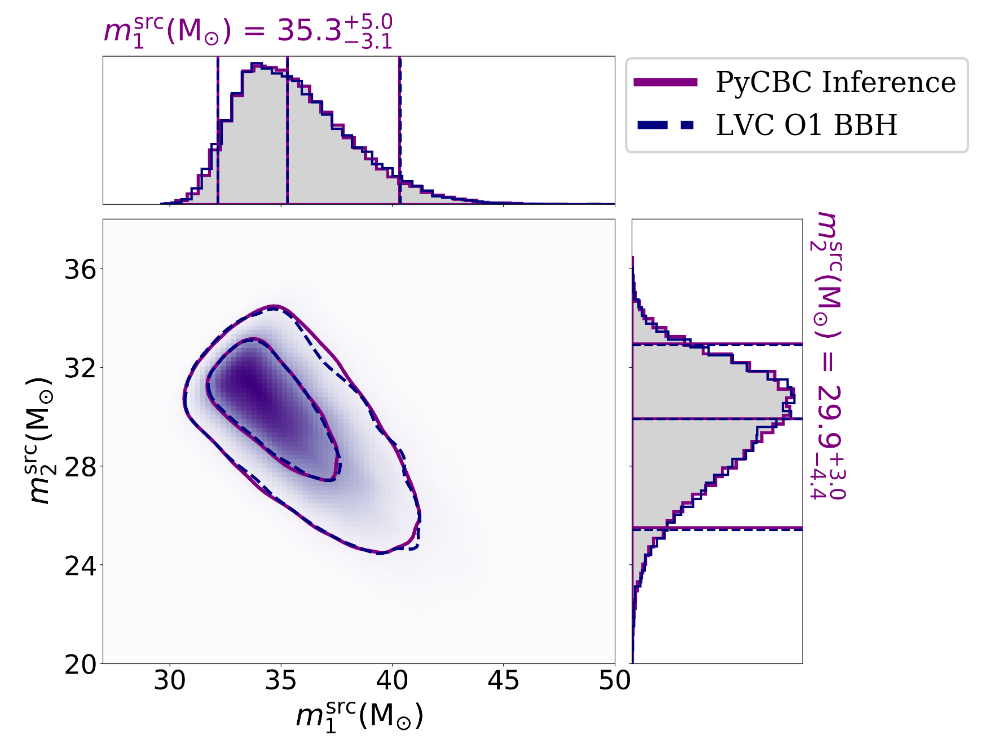
\includegraphics[width=2.5in]{Images/corner_example}
    \caption*{Example of posterior distrubution of masses for GW150914 (arXiv:1807.10312)}
  \end{figure}
}

\section{Neutron Star Mergers and Kilonovae}

\frame{ \frametitle{Neutron Star Mergers and Kilonovae}
  \begin{columns}[c]
    \column{2.5in}
    \begin{itemize}
      \item Neutron stars are the smallest, densest stars \pause
      \item Binary neutron star (BNS) mergers produce gravitational waves \pause
      \item Kilonovae - supernova-like explosions resulting from BNS mergers - are a primary candidate for the creation of heavy elements in the universe, through r-process nucleosynthesis \pause
    \end{itemize}
    \column{2.0in}
    \begin{figure}
      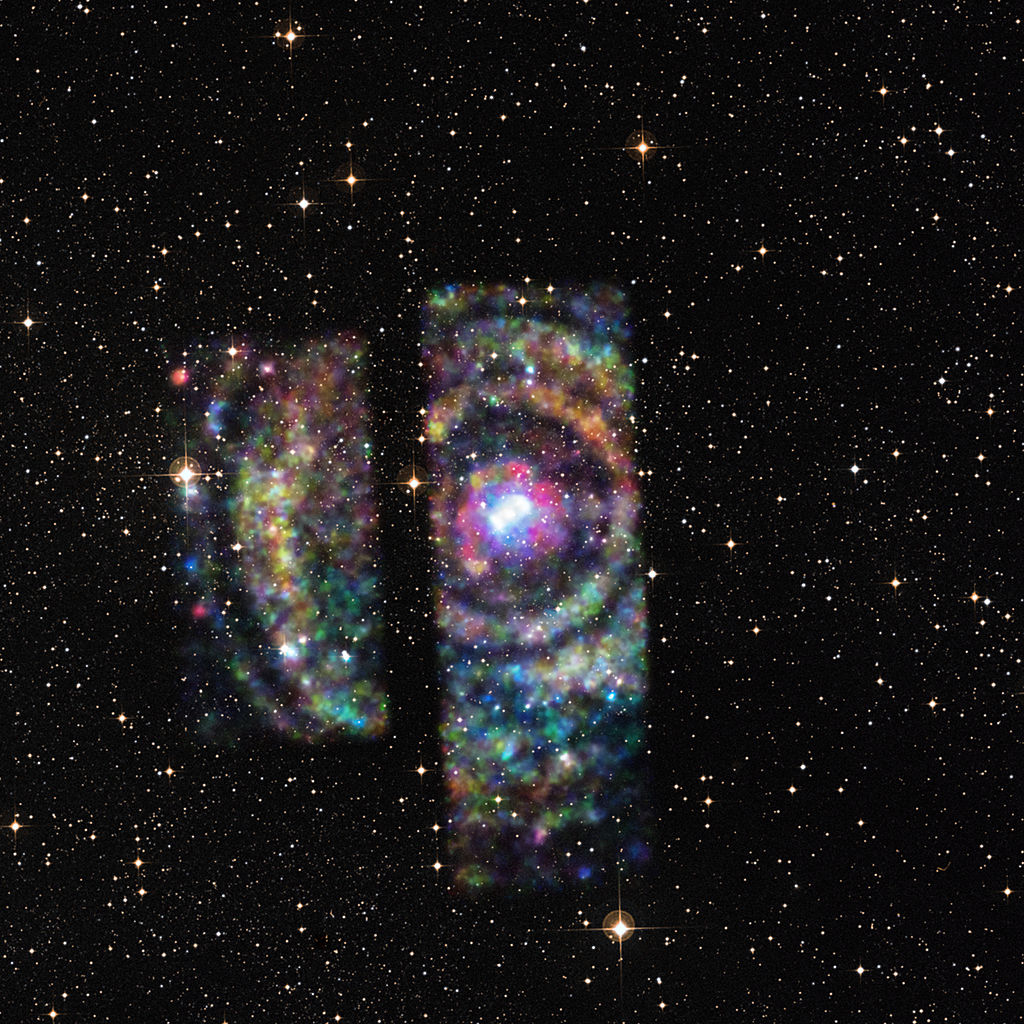
\includegraphics[width=2.0in]{Images/bns_image}
      \caption*{X-ray light rings from a binary neutron star}
    \end{figure}
  \end{columns}
}

\frame{ \frametitle{Multimessenger Astrophysics}
  \begin{columns}[c]
    \column{2.5in}
    \begin{itemize}
      \item Kilonovae produce electromagnetic (EM) transients through the radioactive decay of ejected material \pause
      \item These EM signals can be observed and used in the analysis of BNS mergers \pause
      \item GW170817: first BNS merger detected by LIGO, accompanied by electromagnetic observations across frequency bands \pause
    \end{itemize}
    \column{2.25in}
    \begin{figure}
      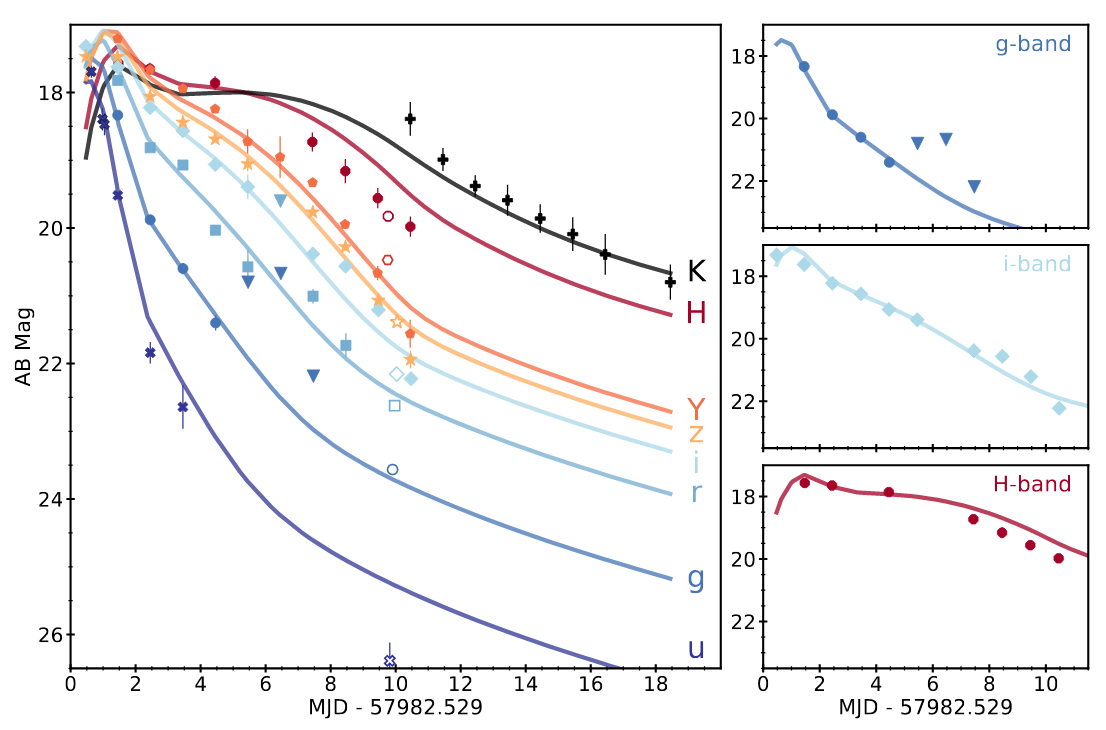
\includegraphics[width=\linewidth]{Images/lightcurves}
      \caption*{GW170817 lightcurves (arXiv:1710.05840)}
    \end{figure}
  \end{columns}
}

\section{GW/EM PE}

\frame{ \frametitle{EM Parameter Estimation}
  \begin{itemize}
    \item Parameter estimation using EM data channels is similar to gravitational wave parameter estimation \pause
    \item Likelihood function used for EM parameter estimation: the log-likelihood of parameter vector $\vec \theta$ is
    \begin{align*}
      \ln L = -0.5 \sum \frac {(x(t) - m(t | \vec \theta))^2} {\Delta x(t)^2 + \Delta m(t | \vec \theta)^2}
    \end{align*}
    where $x(t)$ is the lightcurve magnitude at time $t$, $m(t | \vec \theta)$ is the model value at time $t$ given the current model parameters, $\Delta x(t)$ is the data error, and $\Delta m(t | \vec \theta)$ is the model error.
  \end{itemize}
}

\begin{frame}[fragile] \frametitle{\texttt{EM\_PE}: Rapid Parameter Estimation for EM Transients}
  \begin{columns}[c]
    \column{2.0in}
    \begin{itemize}
      \item Open-source \texttt{Python} package: \texttt{github.com/bwc3252/EM\_PE} \pause
      \item Parameter estimation for arbitrary models and data channels \pause
      \item Uses adaptive Monte Carlo integration to sample parameter space \pause
      \item Functionality: \pause
      \begin{itemize}
        \item Full PE \pause
        \item Visualization of results \pause
        \item Likelihood function for use in other PE codes \pause
      \end{itemize}
    \end{itemize}
    \column{3.0in}
    \begin{verbatim}
    from em_pe import sampler

    ### setup
    dat = "./"
    m = "two_comp"
    f = ["H.txt"]
    out = ""
    params = {...}

    s = sampler(dat, m, f, out)
    lnL = s.log_likelihood(params)
    \end{verbatim}
  \end{columns}
\end{frame}

\frame{ \frametitle{Example for Synthetic Data}
  Parameter recovery for synthetic EM data:
  \begin{columns}[c]
    \column{2.5in}
      \begin{figure}
        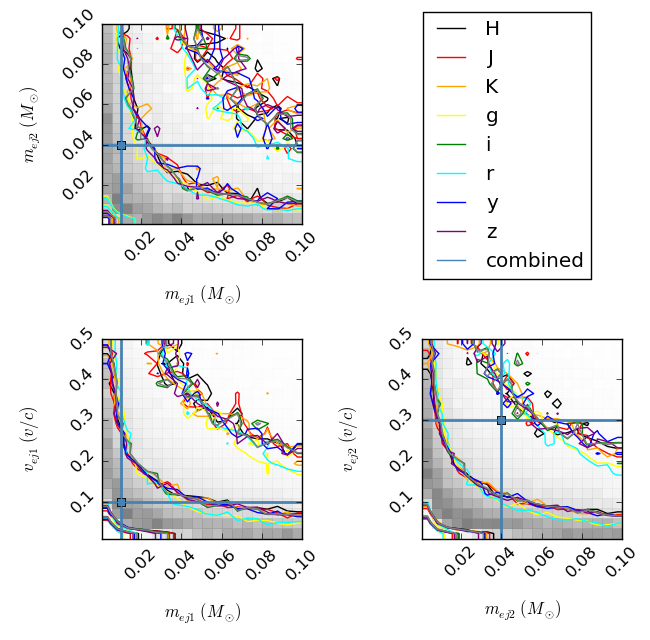
\includegraphics[width=\linewidth]{Images/syn_combined_corner_poster}
      \end{figure}
    \column{2.5in}
    \begin{figure}
      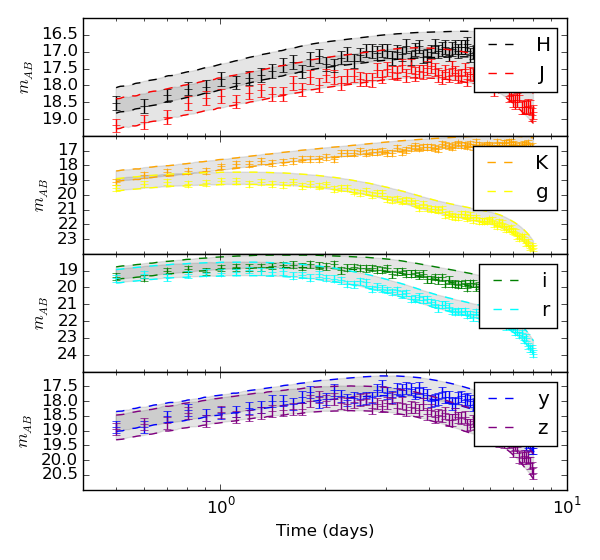
\includegraphics[width=\linewidth]{Images/lc_synthetic}
    \end{figure}
  \end{columns}
}

\frame{ \frametitle{Ongoing Work}
  \begin{itemize}
    \item Joint parameter estimation: PE using both gravitational wave and electromagnetic data \pause
    \begin{itemize}
      \item Combined likelihood: $\ln L = \ln L_{GW} + \ln L_{EM}$ \pause
      \item Different data channels == different constraints on parameters \pause
    \end{itemize}
    \item Combining parameters \pause
    \begin{itemize}
      \item Kilonova ejecta parameters in terms of BNS parameters \pause
    \end{itemize}
    \item Adding new and more complex models \pause
    \item Optimizing PE codes \pause
    \begin{itemize}
      \item GPUs, parallel computing, ...
    \end{itemize}
  \end{itemize}
}

\section{Conclusion}

\frame{
  Questions?
  \begin{figure}
    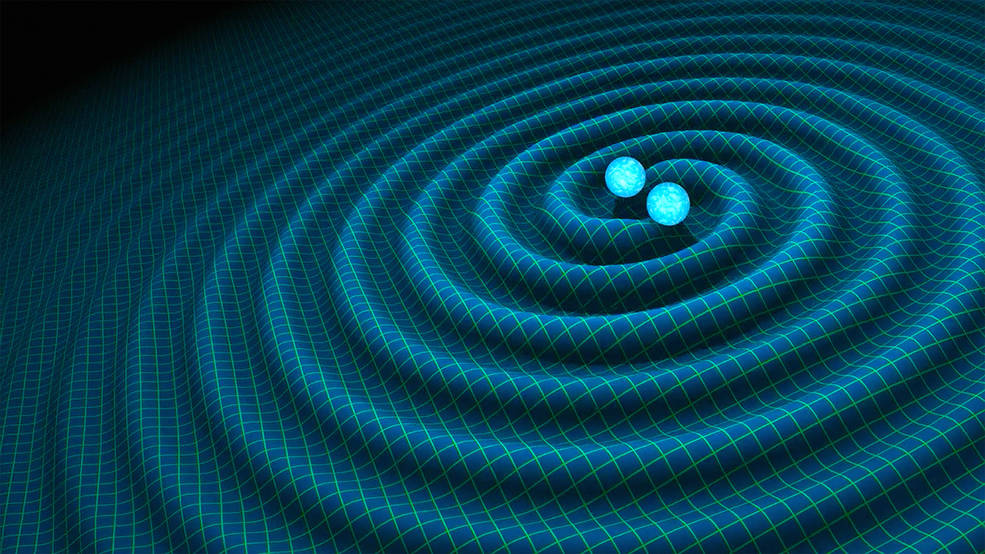
\includegraphics[width=\linewidth]{Images/gw}
    \caption*{Image from R. Hurt/Caltech-JPL}
  \end{figure}
}

\end{document}
